%\documentclass[11pt,a4paper]{article}
%\documentclass[conference]{IEEEtran}
%\documentclass[5pt,conference,letterpaper]{IEEEtran}
\documentclass[conference]{IEEEtran}
\usepackage{graphicx}
\usepackage[hyphens]{url}
% uncomment according to your operating system:
% ------------------------------------------------
%\usepackage[latin1]{inputenc}    %% European characters can be used (Windows, old Linux)
\usepackage[utf8]{inputenc}     %% European characters can be used (Linux)
%\usepackage[applemac]{inputenc} %% European characters can be used (Mac OS)
% ------------------------------------------------
\usepackage[T1]{fontenc}   %% get hyphenation and accented letters right
\usepackage{mathptmx}      %% use fitting times fonts also in formulas
% do not change these lines:
\pagestyle{empty}                %% no page numbers!
%\usepackage[left=35mm, right=35mm, top=15mm, bottom=20mm, noheadfoot]{geometry}
\usepackage{subfig}
\usepackage{multiFloats}
\usepackage{caption}
\usepackage{wrapfig}
\usepackage{listings}
\usepackage{authblk}
\usepackage{todonotes}
\usepackage{float}

\renewcommand\Authfont{\small}
%\renewcommand\Affilfont{\itshape\footnotesize}

\IEEEoverridecommandlockouts
%\makeatother
% begin the document
\begin{document}
%\thispagestyle{empty}
%\sloppy

\title{\textbf{Tools and data integration for eScience platforms}}
\author[1]{Romulo Goncalves}
\author[1]{Niels Drost}
\author[1]{Stefan Verhoeven}
\author[1]{Jisk Attema}
\author[1]{Jason Maassen}

\affil[1]{NLeSC Amsterdam, The Netherlands \vspace{1pt} \{\emph{\{r.goncalves,n.drost,s.verhoeven,j.attema,j.maassen\}@esciencecenter.nl}\}}%, o.rubi\}@esciencecenter.nl}\}}


\date{} % <--- leave date empty
\maketitle\thispagestyle{empty} %% <-- you need this for the first page

\begin{abstract}
\end{abstract}

\section{Introduction}
\label{introduction}

The tools and data integration work of Sherlock project aims to provide easy and efficient data injection
into a HDFS cluster, batch processing, interactive processing and export of results to external processing
or storage systems. The decision to use HDFS as a data hub is due to its utilization in Hansken, NFI system
for forensic research, but also to exploit current state-of-the-art solutions for Big Data exploration such
as Spark. The diagram in Figure 2 shows how each component is interlinked with a Hadoop 2.0 cluster. It has
a data import docker to convert different file types to the most appropriated file format supported by Hadoop.

The choice of its format is based on the type of processing with the aim to improve processing efficiency
and have a low storage footprint. To exploit data locality and fault-tolerance on a Hadoop Cluster, external
libraries are dockerized and through MRdocker, it instantiates a docker image in the Map phase of a MapReduce
job, or SprDocker, it instantiates a docker image on each data node, are executed. The input, the intermediate,
or the final result is made accessible through the Scala, the R, and the Python interfaces of Spark for a
step-wise forensic exploration. Such interfaces allow the users to develop web-apps using R-shiny, or Python
fask to feed Java Script web-pages. It provides a user-friendly visualization with all the heavy computations
being done by Spark. In case the user wants to process intermediate results somewhere else, a bridge through
a NFS mount or through a specialized data exporter is provided by our solution. For example, it allows the
data to be loaded into external database for later re-use or be consumed by an external data visualization
tool running in a docker. 

The remainder of the paper is as follows. Section~\ref{current_approaches} discusses the general
architecture. In Section~\ref{data_exploration}, through different use case scenarios, flexibility
and efficiency on exploring climate and geo-spatial data is shown. Finally the article ends with
a summary in Section~\ref{conclusion} and future plans in Section~\ref{future_plans}.

\section{Background}
\label{background}

\subsection{Forensics eco-system}
One of the challenges encountered every day on forensic research is the large and heterogeneous collection
of libraries, tools, and data available to us. Our project designs and prototypes solutions for the
integration of many existing components into a single system which is flexible, robust and effective for
forensic data exploration.

External libraries have may years of domain knowledge which is not easily converted into a
realtional query. They are part of a long and complex pipe-line which can't all be replaced
by a relational or a series of relational queries. The access to external repositories to
consume data and feed results back to visualization tools or data services turns the
conversion of the pipeline into series of relational queries even more complex.

\subsection{Hadoop eco-system}

\begin{figure}[lb]
%\vspace*{-5mm}
\centering
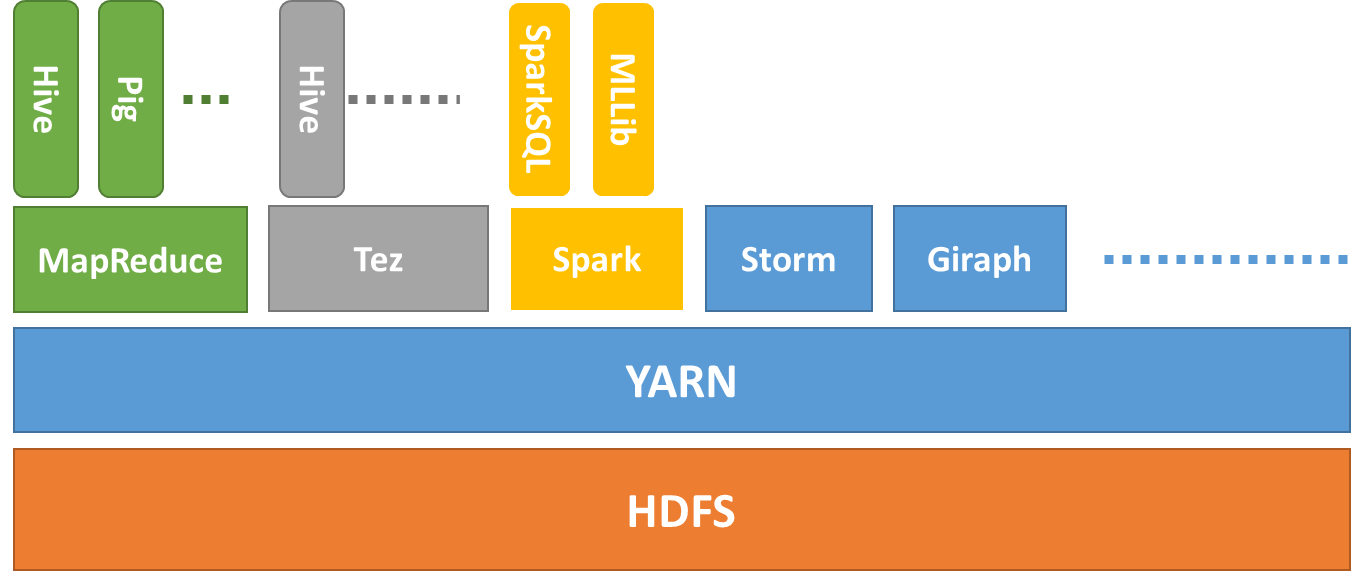
\includegraphics[width=.48\textwidth]{fig/hadoop_2.png}
\caption{Hadoop 2.0}
\label{haddop_2}
\end{figure}


\subsection{Docker Containers}
Docker combines an easy-to-use interface to Linux containers with easy-to-construct image files for those containers. In short, Docker launches very light weight virtual machines.

According to the Docker website, “Docker is an open platform for developers and sysadmins to build, ship, and run distributed applications. Consisting of Docker Engine, a portable, lightweight runtime and packaging tool, and Docker Hub, a cloud service for sharing applications and automating workflows, Docker enables apps to be quickly assembled from components and eliminates the friction between development, QA, and production environments.”, www.docker.com. For more information how how virtualization works and how docker differs from virtual machines check link and its user guide. More info is available at the Docker workshop gitHub.



\section{Architecture}
\label{architecture}

Types of scheduling.

We first use Spark since data is stored in HDFS.
So spark is used to exploit data locality and fault-tolerance.


We schedule different docker containers through spark.
How to connect them using Spark?

Then how other scheduling schemas can be integrated?

Different types of schedulers:
https://www.digitalocean.com/community/tutorials/the-docker-ecosystem-scheduling-and-orchestration

https://docs.docker.com/swarm/scheduler/filter/

Data locality could be questioned and then by using swarm filters we could schedule dockers to
specific locations, however, the scheduling algorithm would be of our responsability.

Keubernet, Spark and Zepplin

http://blog.kubernetes.io/2016/03/using-Spark-and-Zeppelin-to-process-Big-Data-on-Kubernetes.html


How to do it for HDFS cluster, we run docker containers in Spark.

Outside HDFS cluster we use keubernet to schedule docker containers over each node.
A spark cluster can be created, but also a set of containers running othere tools.
Using messos for resource management, several processing tools can co-exist at the same time.

The challenge becomes to access heterogenous data and find a common ground to share data.
The idea is to exploit data vaults when using a DBMS or Spark. Specialized libraries work
with a single data format. They are used often in data preparation phase where classificaiton happens.

Data vaults is not only about importing data, it is also about exporting data.

We are inverting the paradigm with this platform, it is not a DBMS on top of Spark or Hadoop, but both co-exist side by side
where the query plan abstraction goes on level up. With this query interaction is more user friendly, instead of gathering
information we are now extracting knowledge.

When using HDFS, better to use Spark because data locality comes for free.

Using Kubernet it is the first step towards running Spark with access to external file repositories.
For that we will use and extend the latest API released:

In Spark 1.2, we’ve taken the next step to allow Spark to integrate natively with a far larger number of input sources.  These new integrations are made possible through the inclusion of the new Spark SQL Data Sources API.
https://databricks.com/blog/2015/01/09/spark-sql-data-sources-api-unified-data-access-for-the-spark-platform.html

Comparisson between Mesos and Keubernet, fantastic list of differences and why we will pick Keubernet.
http://thenewstack.io/a-brief-comparison-of-mesos-and-kubernetes/


Tricks on how to run spark within containers and be scheduled by Keubernet:
http://www.lshift.net/blog/2015/04/30/swarming-spark/

\section{Orchestration}
\label{orchestration}

We first use Spark since data is stored in HDFS.
So spark is used to exploit data locality and fault-tolerance.
Currently TDI team is working on the integration of other team’s tools using spark\_docker into a concise
workflow. For efficient resource utilization, efficient scheduling while co-existing with other applications
running on the same cluster, TDI team is looking at Mesos and Kubernete. Furthermore, for flexible heterogeneous
data integration and the use of external tables as input data is other direction under consideration where
the data injection stands on the same principles as our internal Data Vaults project.

The map of such workflow into the required resources should be delegated to an outside
systems with a complete overview of the existent ecosystem.

We schedule different docker containers through spark.
How to connect them using Spark?

Then how other scheduling schemas can be integrated?

Different types of schedulers:
%https://www.digitalocean.com/community/tutorials/the-docker-ecosystem-scheduling-and-orchestration

%https://docs.docker.com/swarm/scheduler/filter/

Data locality could be questioned and then by using swarm filters we could schedule dockers to
specific locations, however, the scheduling algorithm would be of our responsability.

Keubernet, Spark and Zepplin
%http://blog.kubernetes.io/2016/03/using-Spark-and-Zeppelin-to-process-Big-Data-on-Kubernetes.html

Comparisson between Mesos and Keubernet, fantastic list of differences and why we will pick Keubernet.
%http://thenewstack.io/a-brief-comparison-of-mesos-and-kubernetes/

\section{System in Action}
\label{system_in_action}


\subsection{Deep Learning}
The Convolutional Neural Networks (CNN) are a type of deep learning networks, Y. Bengio, "Learning deep
architechures for AI". CNNs are a family of multi-layer neural networks particularly designed for use
on two-dimensional data, such as images. For a quick introduction to CNNs, please refer to section 2.3
of the “Large-scale Computer Vision” overview. For a more elaborate introduction, please refer to the
online book “Neural Networks and Deep Learning” and to the vast resources on deeplearning.net.
Sherlock

Image classification in forensics is a very common request by the digital forensic investigators. 

\subsection{Analyzing document corpora}
While searching a device for incriminating evidence, text documents are commonly encountered. Analyzing the
content of such documents is a challenging task which would require investigators to read through large volumes
of text, without any information to guide them through the search. What is this document about? How does it
relate to other documents? Are there any trends amongst them? Do I need to read through this pile of documents?
Or could I spot a particular document which is more interesting than the rest?

We will tackle these problems using natural language processing tools. The aim of this group is to use NLP
tools to group documents with similar content and provide investigators with the tools to quickly gain insight
into large collections of text.

In the field of Natural Language Processing (NLP), topic modeling has become a popular technique for analyzing
large sets of documents. Topic models attempt to infer a set of topics (basically, bags of words) and then
identify the probability of a topic being contained in a document (e.g. Document1 is made up of 0.5 * Football
topic + 0.2 * General sports topic + 0.3 * Drugs and crime topic).

However there are still many open questions when using topic modeling: document pre-processing, optimum number
of topics to use, visualization and interpretation of the results, etc.

One focus are is investigating techniques for visualizing results from topic models in the most useful and
meaningful way. The ultimate aim is to be able to take a list set of documents (e.g. emails from an inbox)
and cluster them into different groups of similar emails (e.g. emails work, family, leisure). To achieve this
we will need to use existing natural language processing technique, investigate suitable similarity metrics
between documents, and develop (interactive?) visualization techniques.

We will be using the infamous Enron email data set as our document collection.

\section{Future work}
\label{future_work}

Integration of data vaults into Spark.

Access only to Hive Tables.

Monunt external data files as Data Frames.
A DataFrame is a distributed collection of data organized into named columns. It is conceptually equivalent to a table in a relational database or a data frame in R/Python, but with richer optimizations under the hood. DataFrames can be constructed from a wide array of sources such as: structured data files, tables in Hive, external databases, or existing RDDs.

In Spark not possible to make and RDD out of NetCDF.
There are specialized modules for each tool, but the combination of different data sets is not possible.


http://stackoverflow.com/questions/11816609/column-based-or-row-based-for-hbase


http://www.sparkexpert.com/2015/01/02/load-database-data-into-spark-using-jdbcrdd-in-java/

In Spark 1.2, we’ve taken the next step to allow Spark to integrate natively with a far larger number of input sources.  These new integrations are made possible through the inclusion of the new Spark SQL Data Sources API.

https://databricks.com/blog/2015/01/09/spark-sql-data-sources-api-unified-data-access-for-the-spark-platform.html

\section{Future work}

----Towards Generating ETL Processes for Incremental Loading---
We presented an approach for generating
incremental load
processes
for  data  warehouse  refreshment  from
declarative
schema mappings
.  The basis of our work has been provided
by Orchid, a prototype system developed at IBM Almaden
Research Center, that translates
schema mappings
into ETL
processes and vice versa.  Orchid-generated ETL processes,
however,  are  limited  to
initial  load  scenarios
,  i.e.  source
data  is  exhaustively  extracted  and  the  warehouse  is  com-
109
pletely  (re)built.   Incremental  load  processes,  in  contrast,
propagate changes from the sources to the data warehouse.
This approach has clear performance benefits.  Change Data
Capture (CDC) and Change Data Application (CDA) tech-
niques  are  used  to  capture  changes  at  the  sources  and  re-
fresh the data warehouse, respectively.  We defined a model
for
change  data
to  characterize  both,  the  output  of  CDC
techniques  and  the  input  of  CDA  techniques.   Since  CDC
techniques may su from limitations we introduced a no-
tion of
partial  change  data
.  We discussed the propagation
of  partial  change  data  within  incremental  load  processes.
Our  approach  allows  for  reasoning  on  how  limitations  of
CDC techniques determine the set of applicable CDA tech-
niques.  That is, it allows inferring satisticable CDA reuire-
ments from given CDC limitations and, the other way round,
acceptable CDC limitations from given CDA requirements.
We further, demonstrated the exploitation of properties of
data sources (such as schema constraints) to reduce the com-
plexity  of  incremental  load  processes.   By  leveraging  Or-
chid's  deployment  facilities,  we  are  able  to  generate  exe-
cutable  ETL  processes.   We  are  confident  that  our  work
contributes to the improvement of ETL development 




\section{Summary}
\label{summary}


{%\footnotesize
\bibliographystyle{abbrv}
\bibliography{references}
}

\end{document}
